% LATEX TYPEWRITER DOCUMENT MODEL A --------------------------- 80 CHARACTERS :

% ---------------------------------------------------------------- PARAMETERS :

\documentclass[12pt,landscape]{article}
% document in A3 horizontal
\usepackage[margin=2cm,a3paper]{geometry}% http://ctan.org/pkg/geometry
% pics
\usepackage{graphicx} 
% background on all pages
\usepackage[pages=all]{background}

\backgroundsetup{
scale=1,
color=black,
opacity=1,
angle=0,
contents={%
  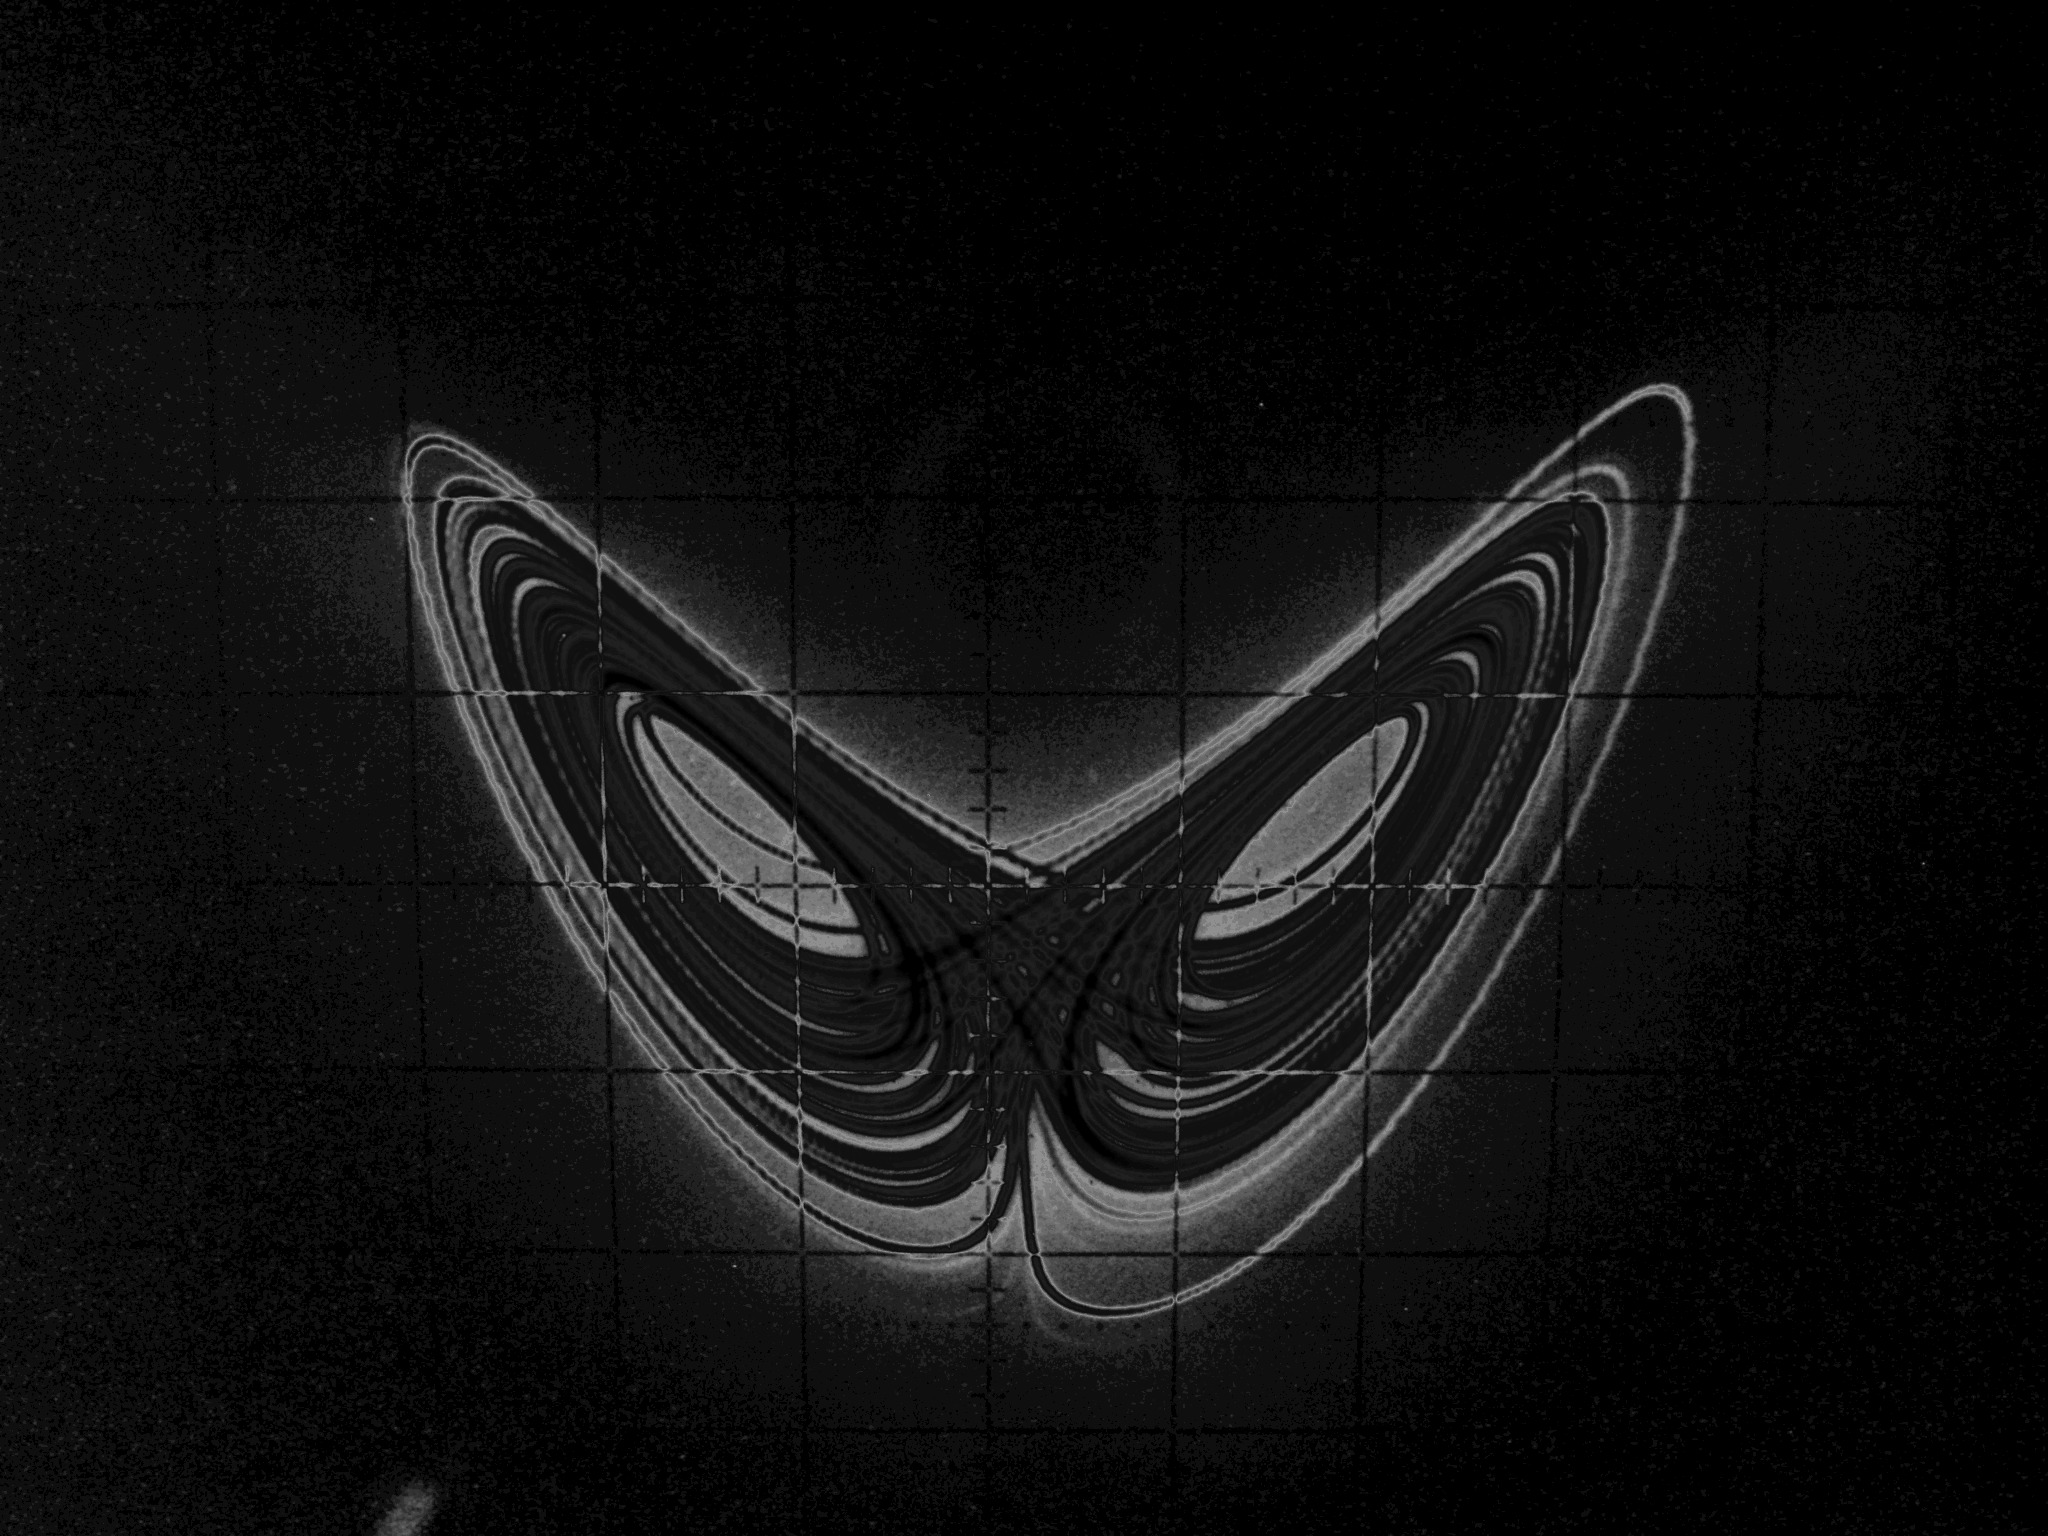
\includegraphics[width=\paperwidth,height=\paperheight]{lorenz.jpg}
  }%
}
\usepackage{titlesec}
\titleformat*{\section}{\Huge\bfseries}



% ------------------------------------------------------------------ DOCUMENT :

% Begin the document
\begin{document}
\LARGE
\color{white}
{\tt
\begin{center}

% HERE START THE TEXT ---------------------------------------------------------

\section*{PORTFOLIO}
Luca Spanedda
\newline
2022
\clearpage

% ---------- New Chapter ----------

\section*{Introduction}

Luca Spanedda is a Composer and Musician.
\newline
He was born in Rome on 15th February 1995.
\newline
His attention to music surfs from cybernetics to technologies,
\newline
and from sound and human spaces to social criticism.

\begin{figure}[!htb]
\minipage{0.25\textwidth}
  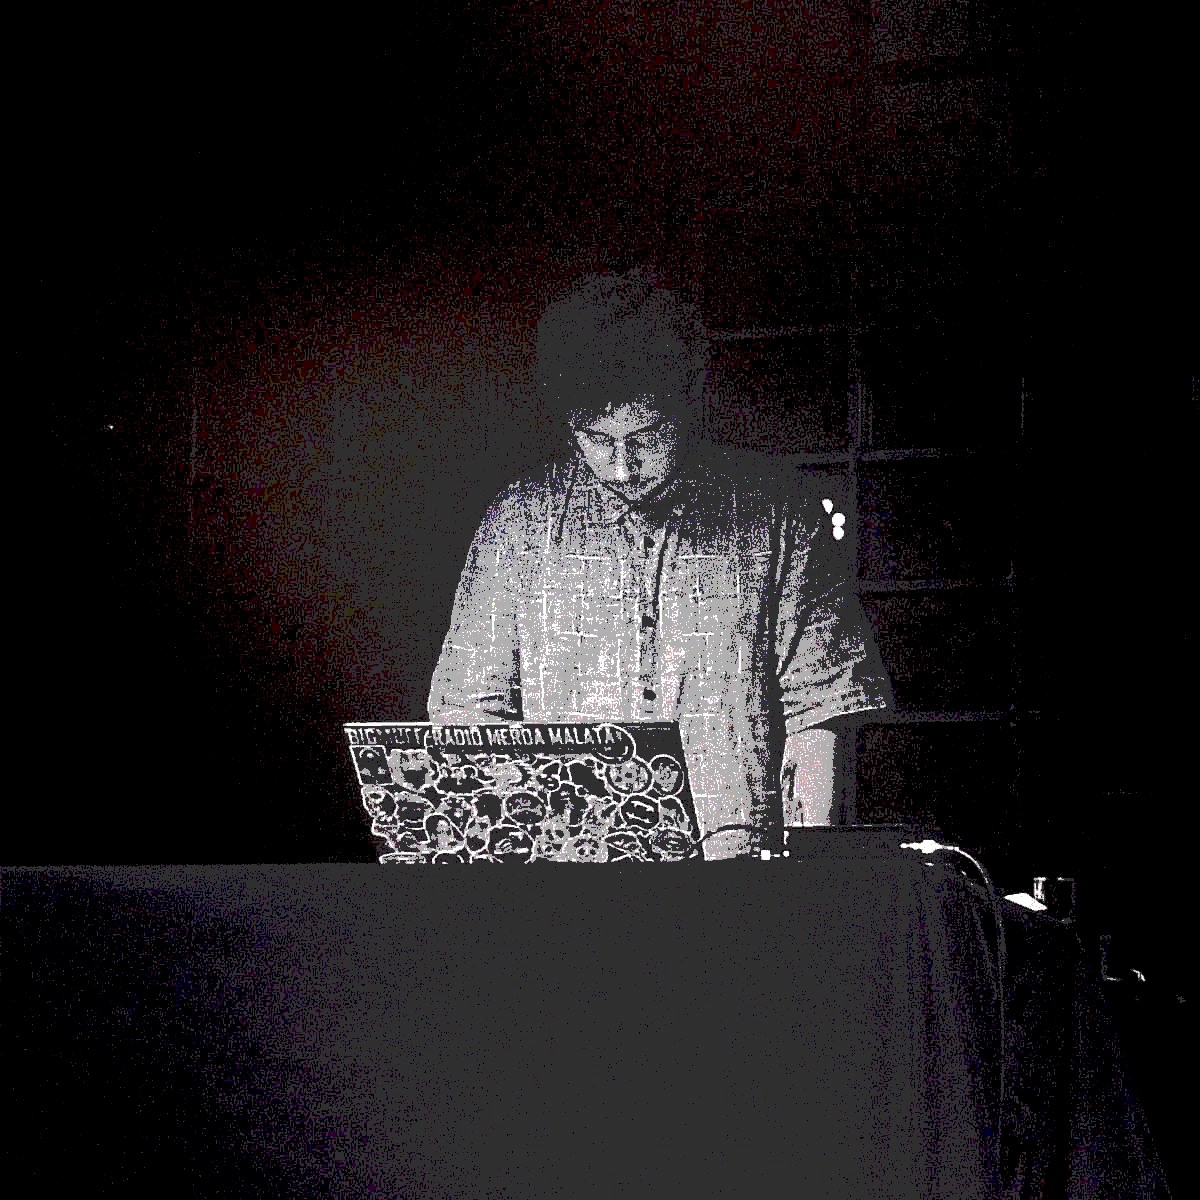
\includegraphics[width=8cm]{portfolio1.jpg}

\endminipage\hfill
\minipage{0.25\textwidth}
  
\includegraphics[width=8cm]{portfolio2.jpg}

\endminipage\hfill
\minipage{0.25\textwidth}%
  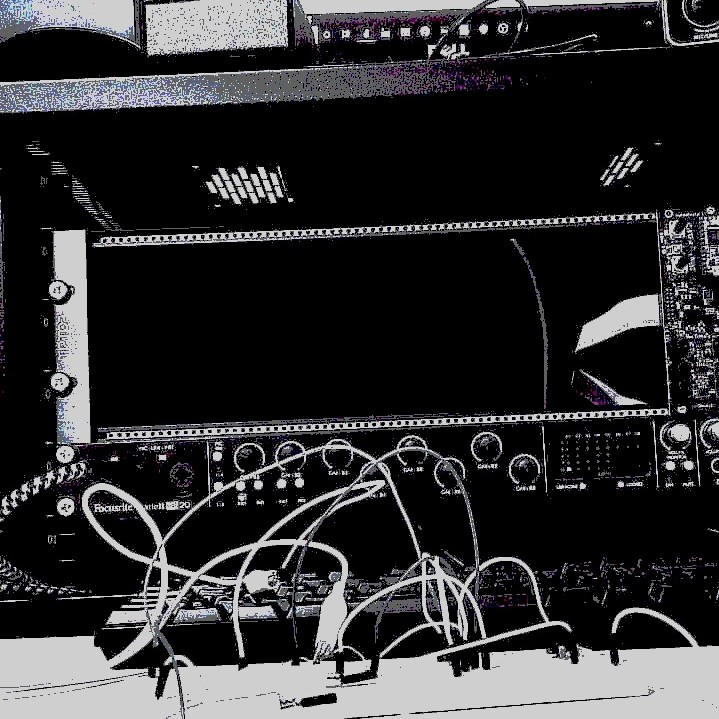
\includegraphics[width=8cm]{portfolio3.jpg}

\endminipage\hfill
\minipage{0.25\textwidth}%
  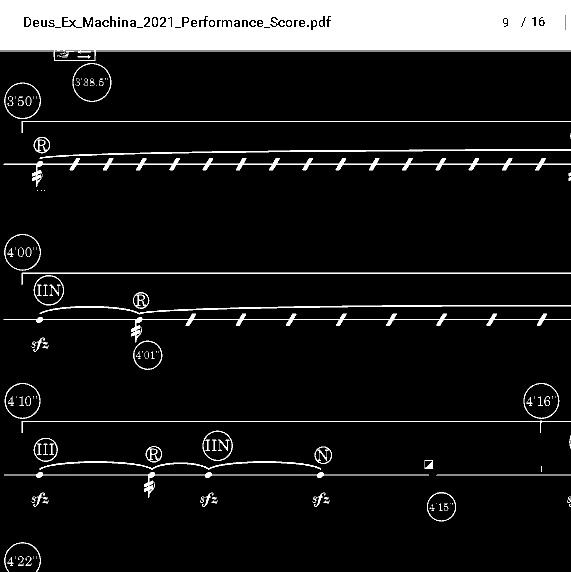
\includegraphics[width=8cm]{portfolio4.jpg}

\endminipage
\end{figure}
\begin{figure}[!htb]
\minipage{0.25\textwidth}
  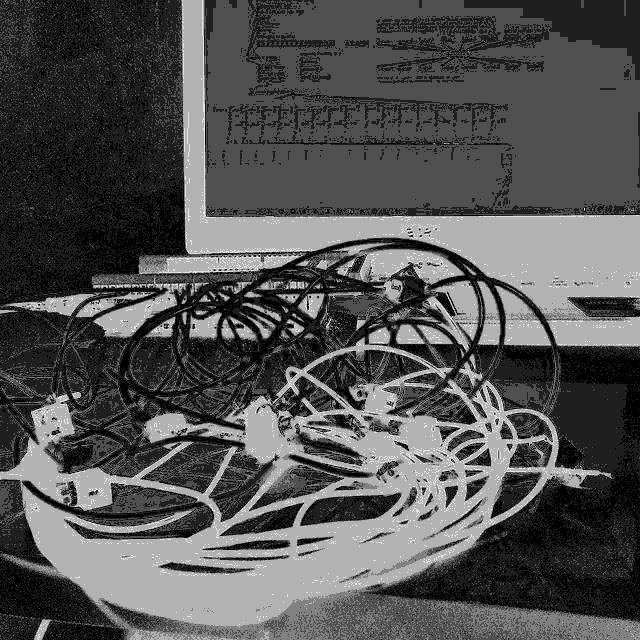
\includegraphics[width=8cm]{jacks.jpg}

\endminipage\hfill
\minipage{0.25\textwidth}
  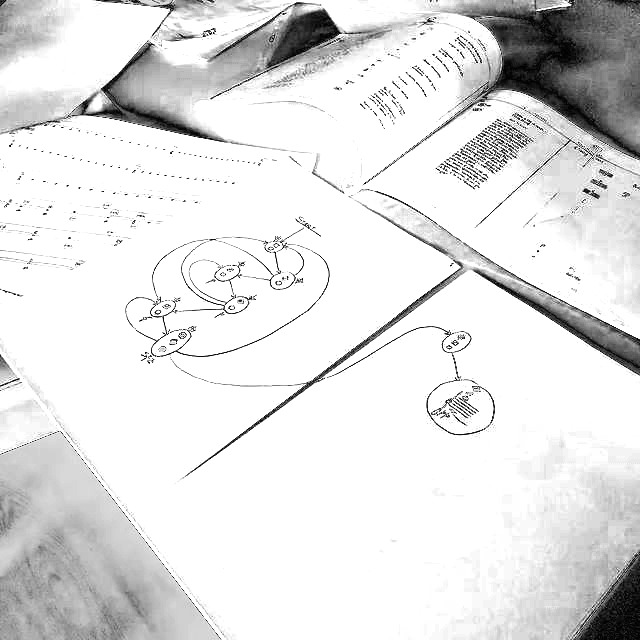
\includegraphics[width=8cm]{sketch.jpg}

\endminipage\hfill
\minipage{0.25\textwidth}%
  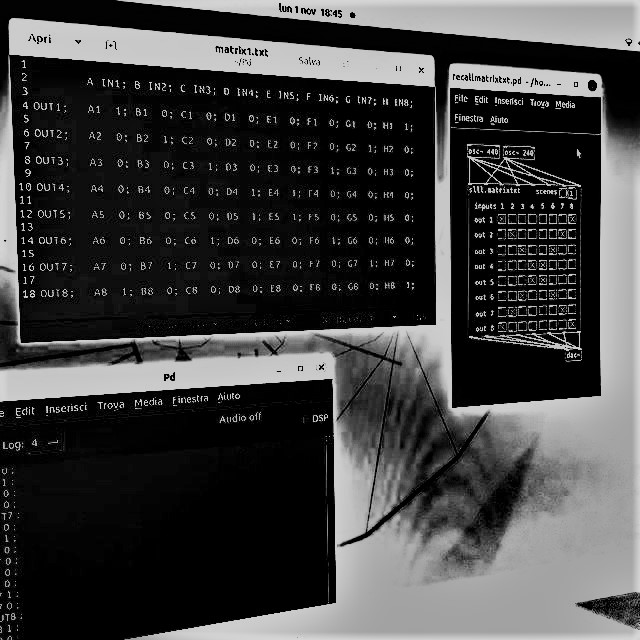
\includegraphics[width=8cm]{pd.jpg}

\endminipage\hfill
\minipage{0.25\textwidth}%
  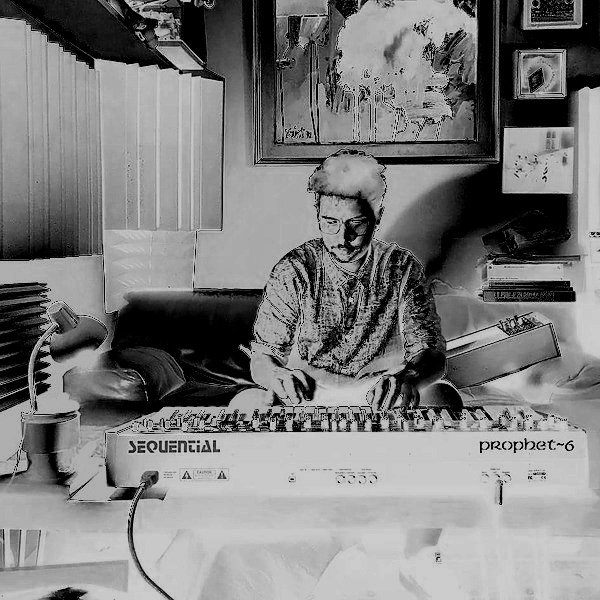
\includegraphics[width=8cm]{proph.jpg}

\endminipage
\end{figure}

\clearpage

% ---------- New Chapter ----------

\section*{Academic Programs}

He graduated in economics, finance and marketing in 2015,
\newline
consequently he began his academic program in electronic music
\newline
at the Santa Cecilia Conservatory of Rome, as a student of electroacoustic composition 
\newline
with the masters Michelangelo Lupone and Nicola Bernardini, 
where he graduated in 2020.
\newline
He is now enrolled in the last two-year course (Biennio)
of Electronic Music at the Conservatory Santa Cecilia in Rome.

\begin{figure}[!htb]
\minipage{0.25\textwidth}
  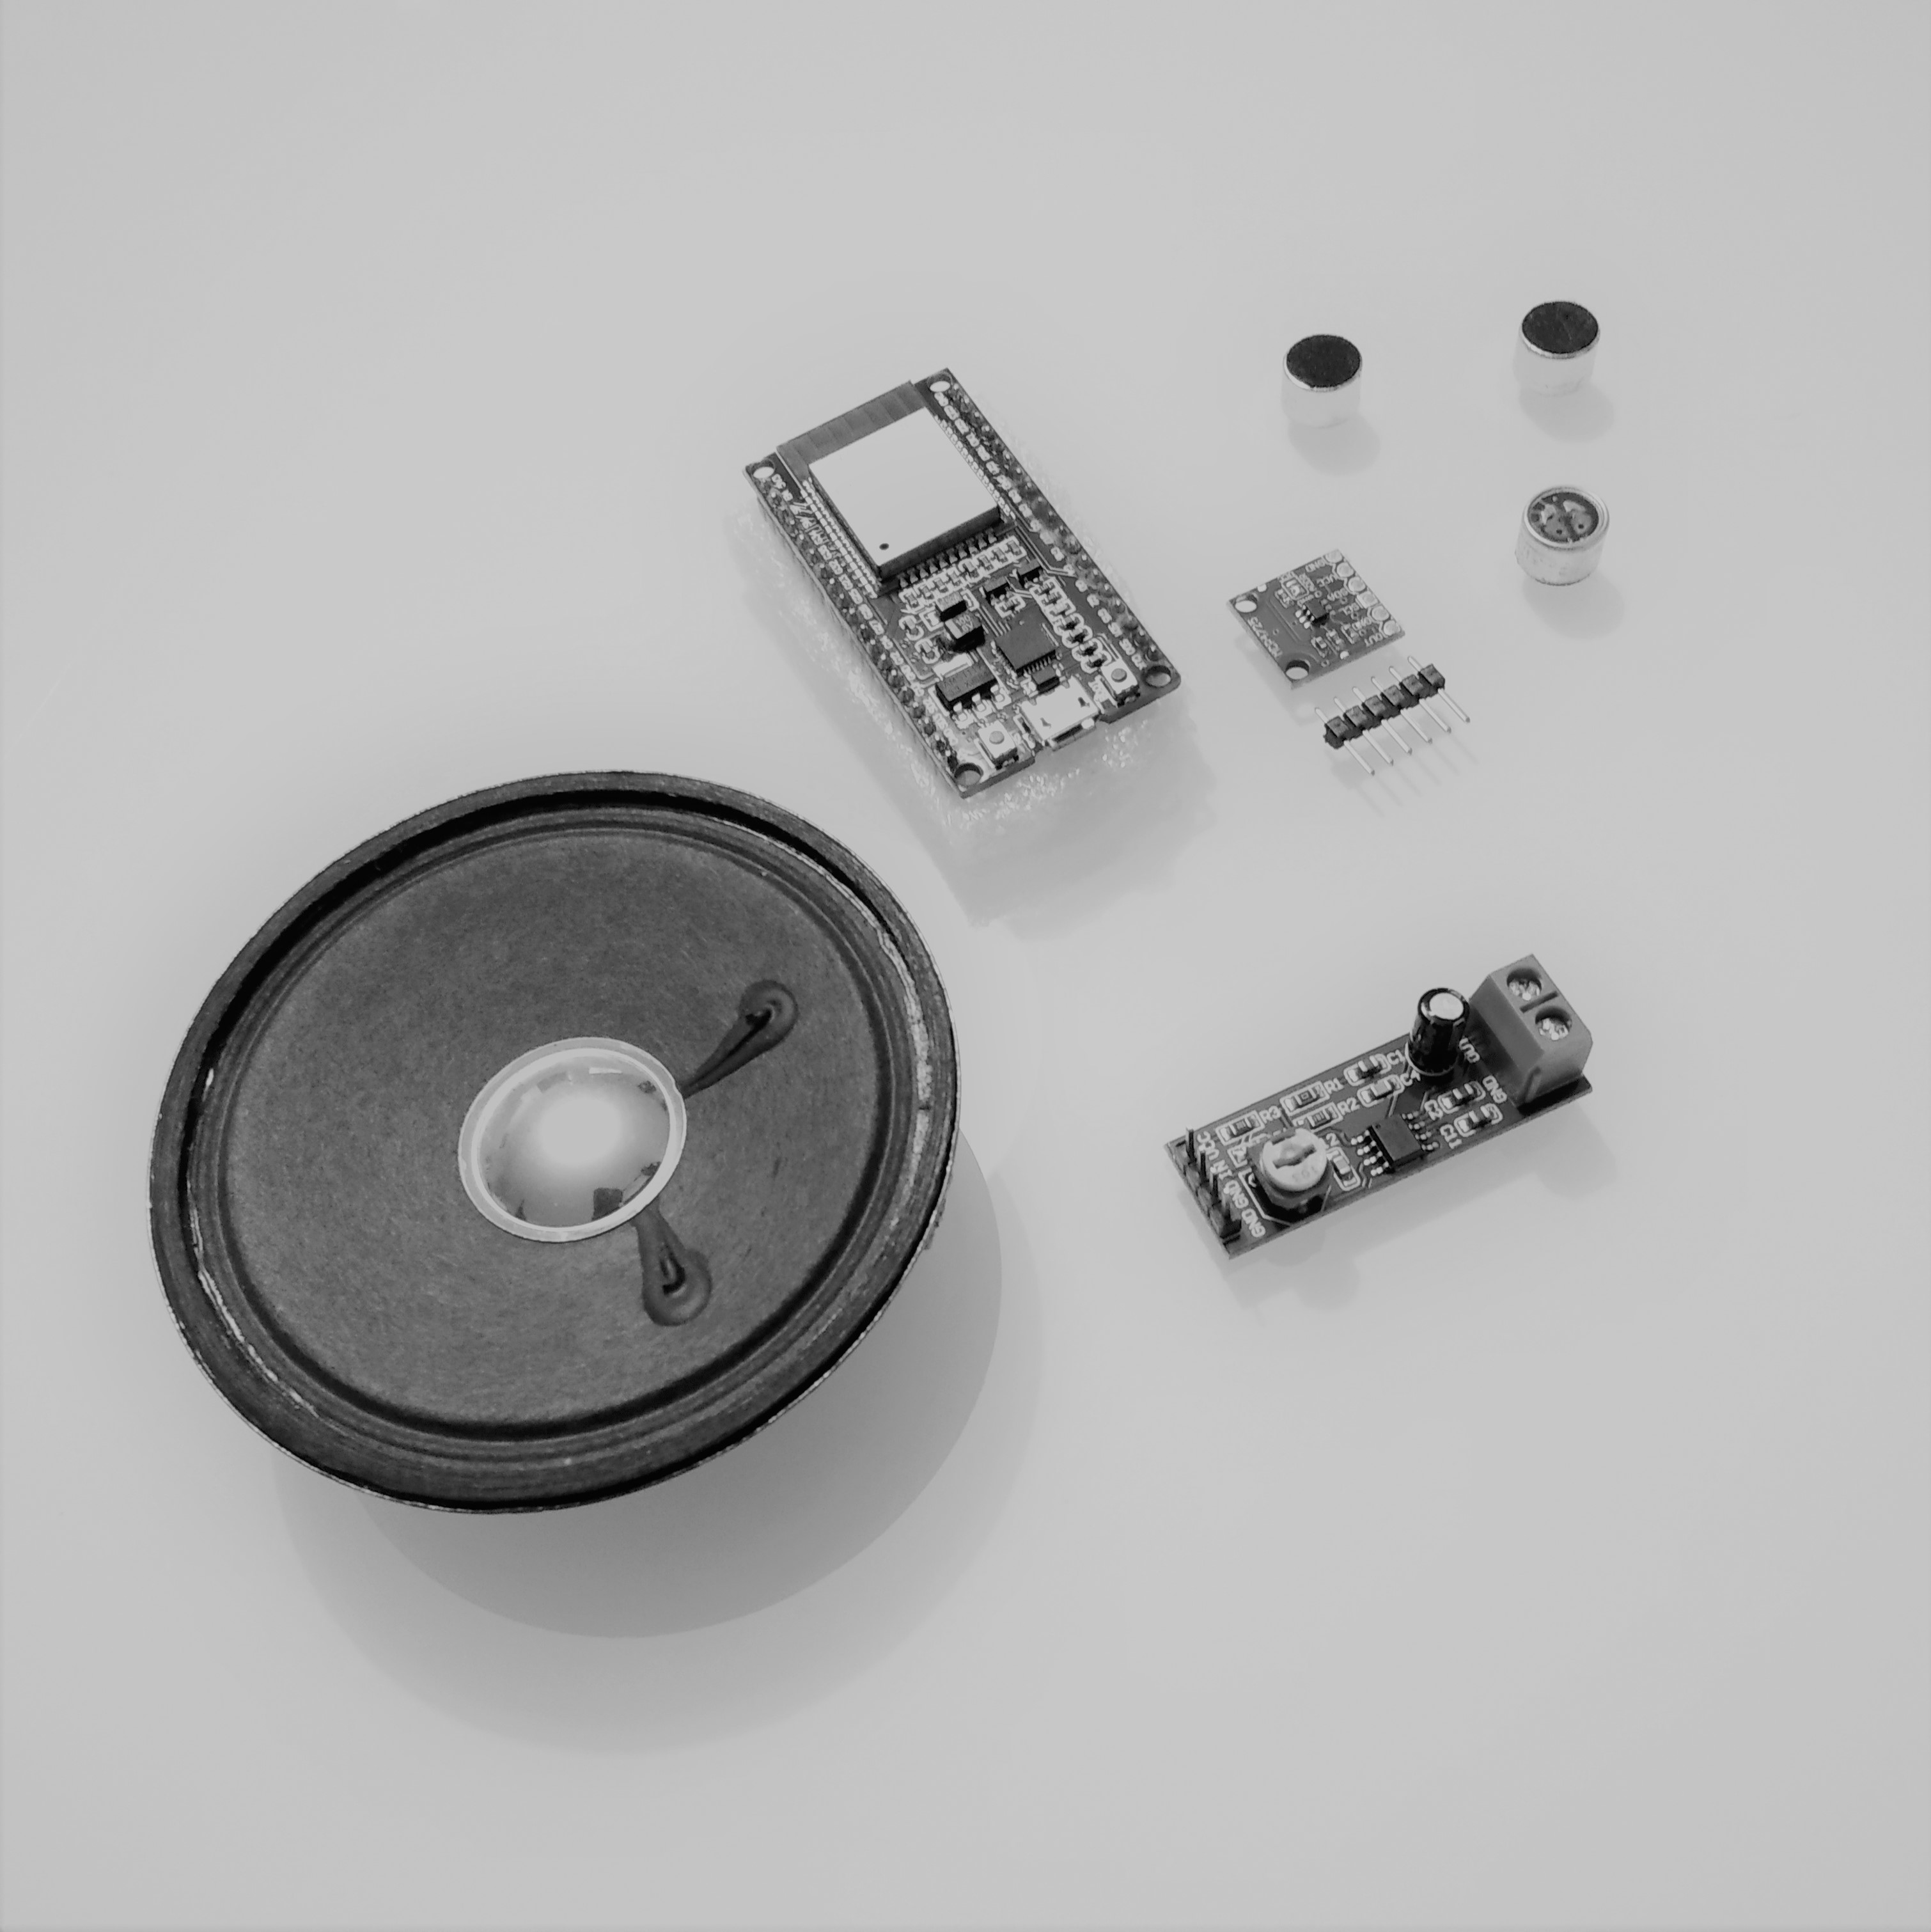
\includegraphics[width=8cm]{electroac1.jpg}

\endminipage\hfill
\minipage{0.25\textwidth}
  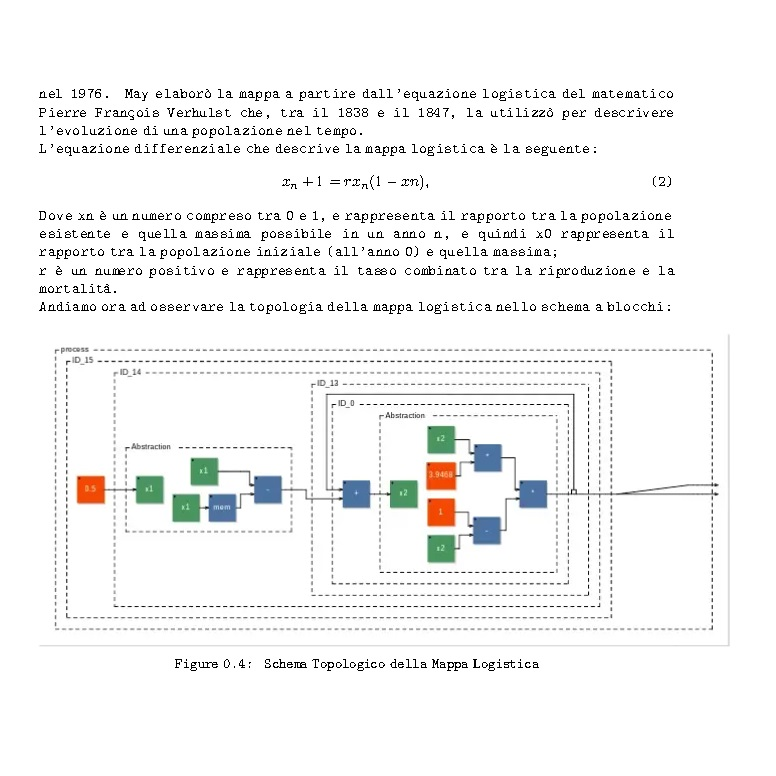
\includegraphics[width=8cm]{info1.jpg}

\endminipage\hfill
\minipage{0.25\textwidth}%
  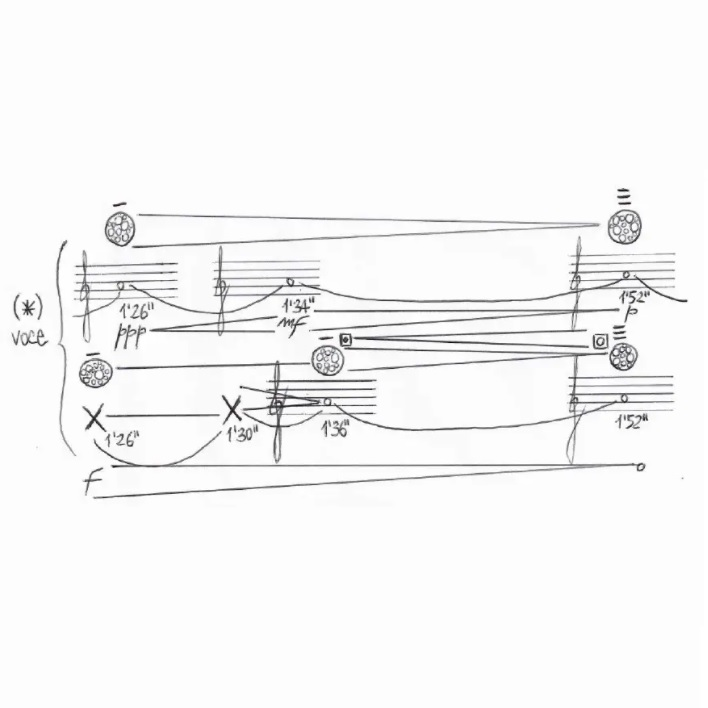
\includegraphics[width=8cm]{threestudies1.jpg}

\endminipage\hfill
\minipage{0.25\textwidth}%
  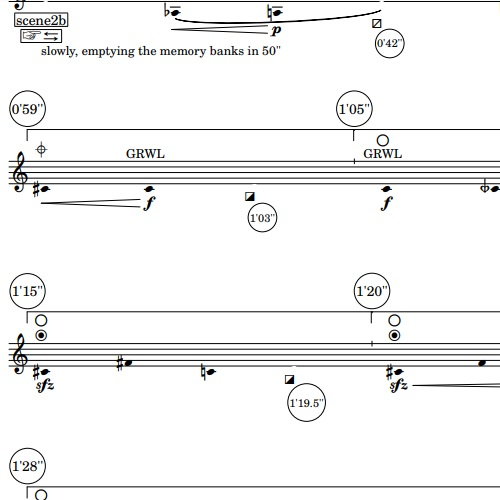
\includegraphics[width=8cm]{deusex1.jpg}

\endminipage
\end{figure}

Participation to various seminars 
held by: 
\newline
Giorgio Netti, Giorgio Nottoli,
Simone Pappalardo, at Conservatorio Santa Cecilia (RM).
\newline
Fondazione Musica per Roma
Dal segno al suono: il lavoro del musicista”. On the occasion of the PMCE concert (Parco della
Musica Contemporanea Ensemble), at Auditorium Parco della Musica (RM).
\newline
And online Classes held by: Grame - FAUST, 
Powland - Powclass with Moon Armada on Build Soundart Devices.

\clearpage

% ---------- New Chapter ----------

\section*{Music for Films}

He wrote some pieces for films such as the
\newline
RAI film "Aquadro", a Stefano Lodovichi's film in 2013 and
\newline
From My House In Da House a Giovanni La Gorga's film in 2021.

\begin{figure}[!htb]
\minipage{0.25\textwidth}
  
\includegraphics[width=8cm]{aquadrocover.jpg}

\endminipage\hfill
\minipage{0.25\textwidth}
  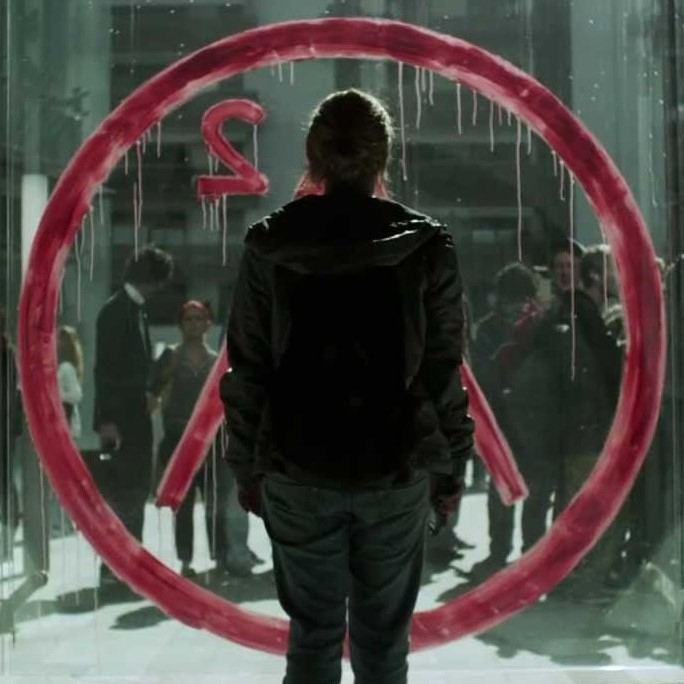
\includegraphics[width=8cm]{aquadroscene.jpg}

\endminipage\hfill
\minipage{0.25\textwidth}%
  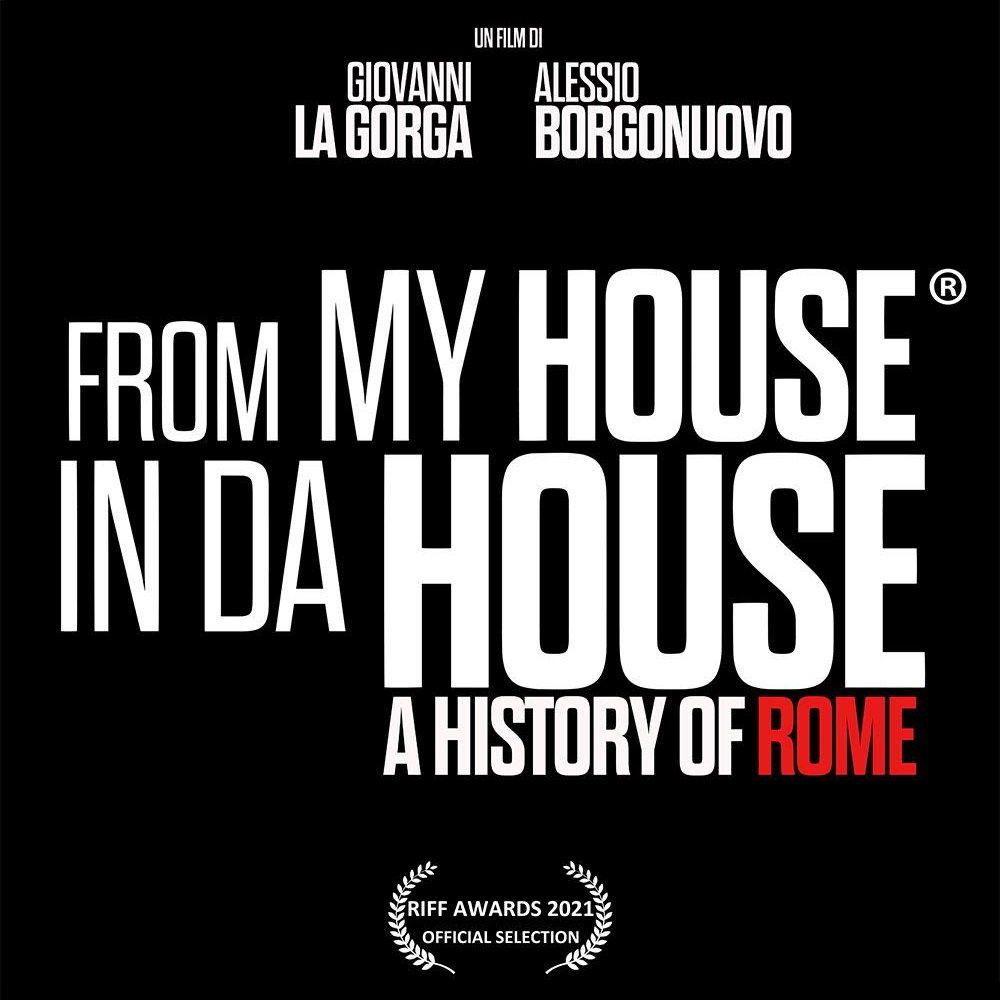
\includegraphics[width=8cm]{frommycover.jpg}

\endminipage\hfill
\minipage{0.25\textwidth}%
  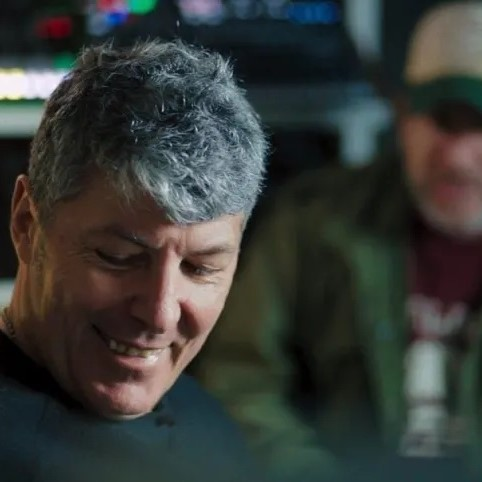
\includegraphics[width=8cm]{frommyscene.jpg}

\endminipage
\end{figure}

\clearpage

% ---------- New Chapter ----------

\section*{Live Performances}

In 2017 he presented "Asteroidi" an audio-visual work,
with the multimedia composition class of M. Riccardo Santoboni at the Master in Sonic Arts
(University of Rome Tor Vergata)
\newline
and at the Academic Hall of the Conservatory Santa Cecilia.
\newline
In 2021, he performed in concert the electronic part
of the Post-prae-ludium n. 1 for Donau by Luigi Nono,
at the Goethe-Institut Italien in Rome, ArteScienza festival.
\newline
And also in 2021 he performs live the LP released by Mossa Records
(independent Roman electronic music label),
at the Klang club in Rome.

\begin{figure}[!htb]
\minipage{0.25\textwidth}
  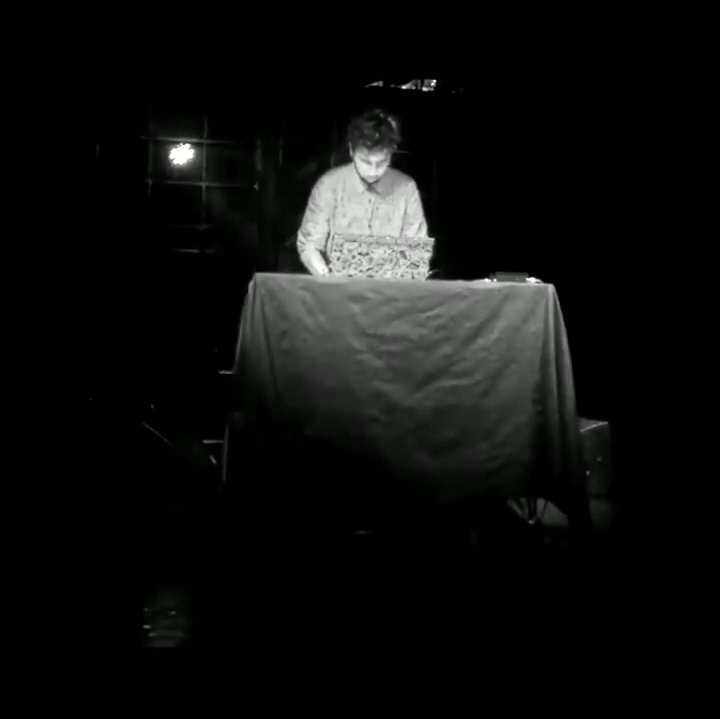
\includegraphics[width=8cm]{live1.jpg}

\endminipage\hfill
\minipage{0.25\textwidth}
  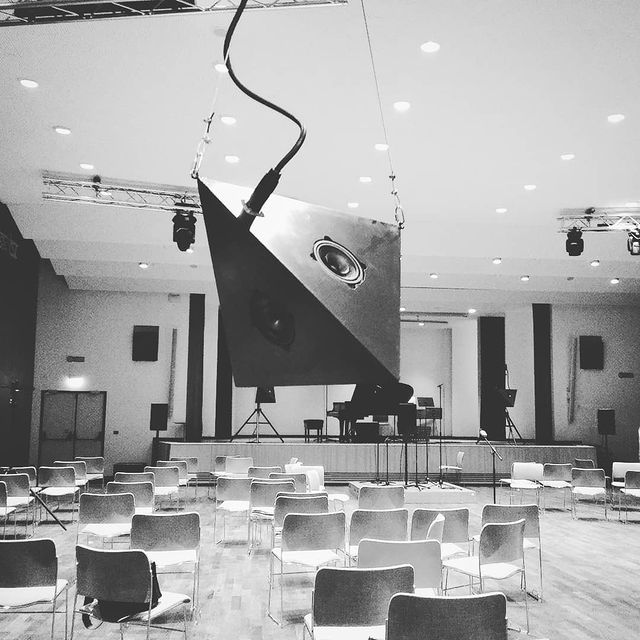
\includegraphics[width=8cm]{live2.jpg}

\endminipage\hfill
\minipage{0.25\textwidth}%
  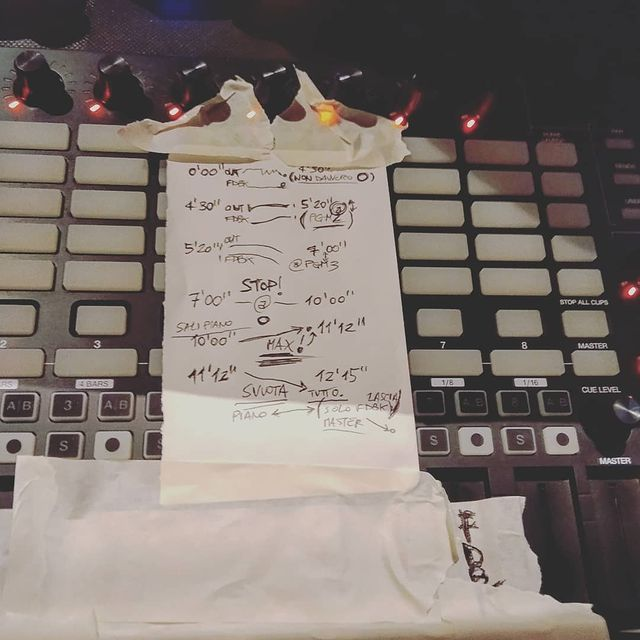
\includegraphics[width=8cm]{live3.jpg}

\endminipage\hfill
\minipage{0.25\textwidth}%
  \includegraphics[width=8cm]{live4.jpg}

\endminipage
\end{figure}

\clearpage

% ---------- New Chapter ----------

\section*{Productions}

He started making music as a teenager,
as a DJ to then turning as a producer,
\newline
in some drum and bass collectives in Rome (IT),
publishing also some LPs.
\newline
He still publish different kinds of electronic
works under the Moniker: Stigma

\begin{figure}[!htb]
\minipage{0.25\textwidth}
  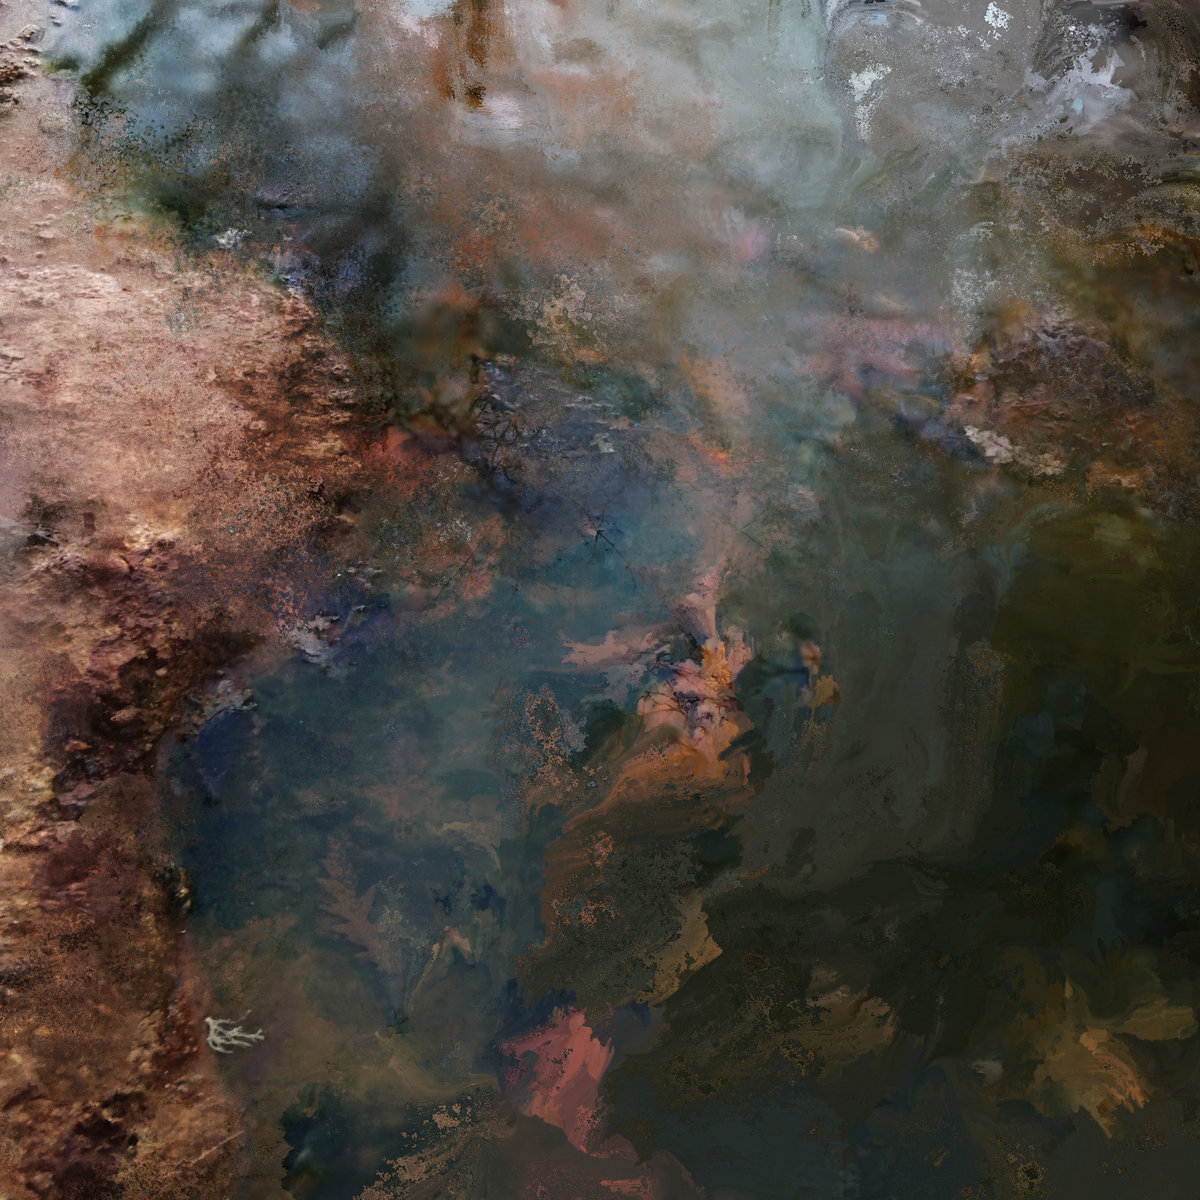
\includegraphics[width=8cm]{particles.jpg}

\endminipage\hfill
\minipage{0.25\textwidth}
  
\includegraphics[width=8cm]{otherside.jpg}

\endminipage\hfill
\minipage{0.25\textwidth}%
  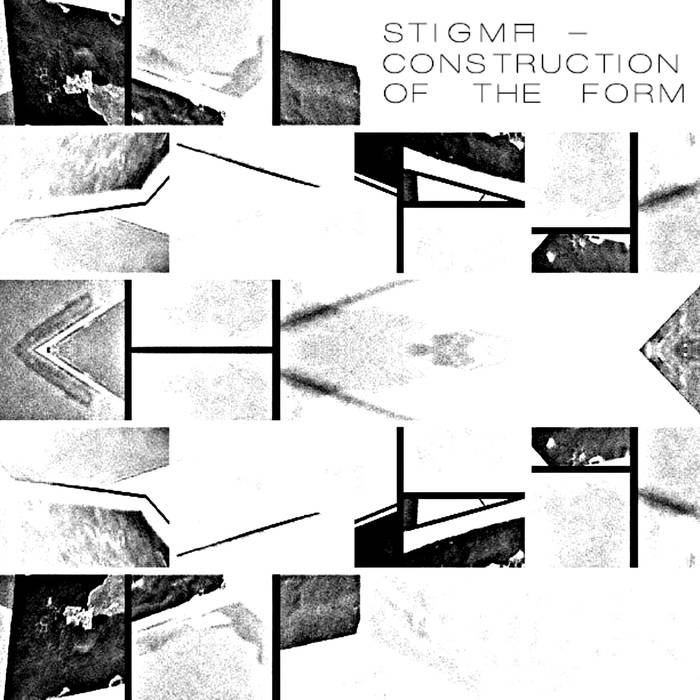
\includegraphics[width=8cm]{construction.jpg}

\endminipage\hfill
\minipage{0.25\textwidth}%
  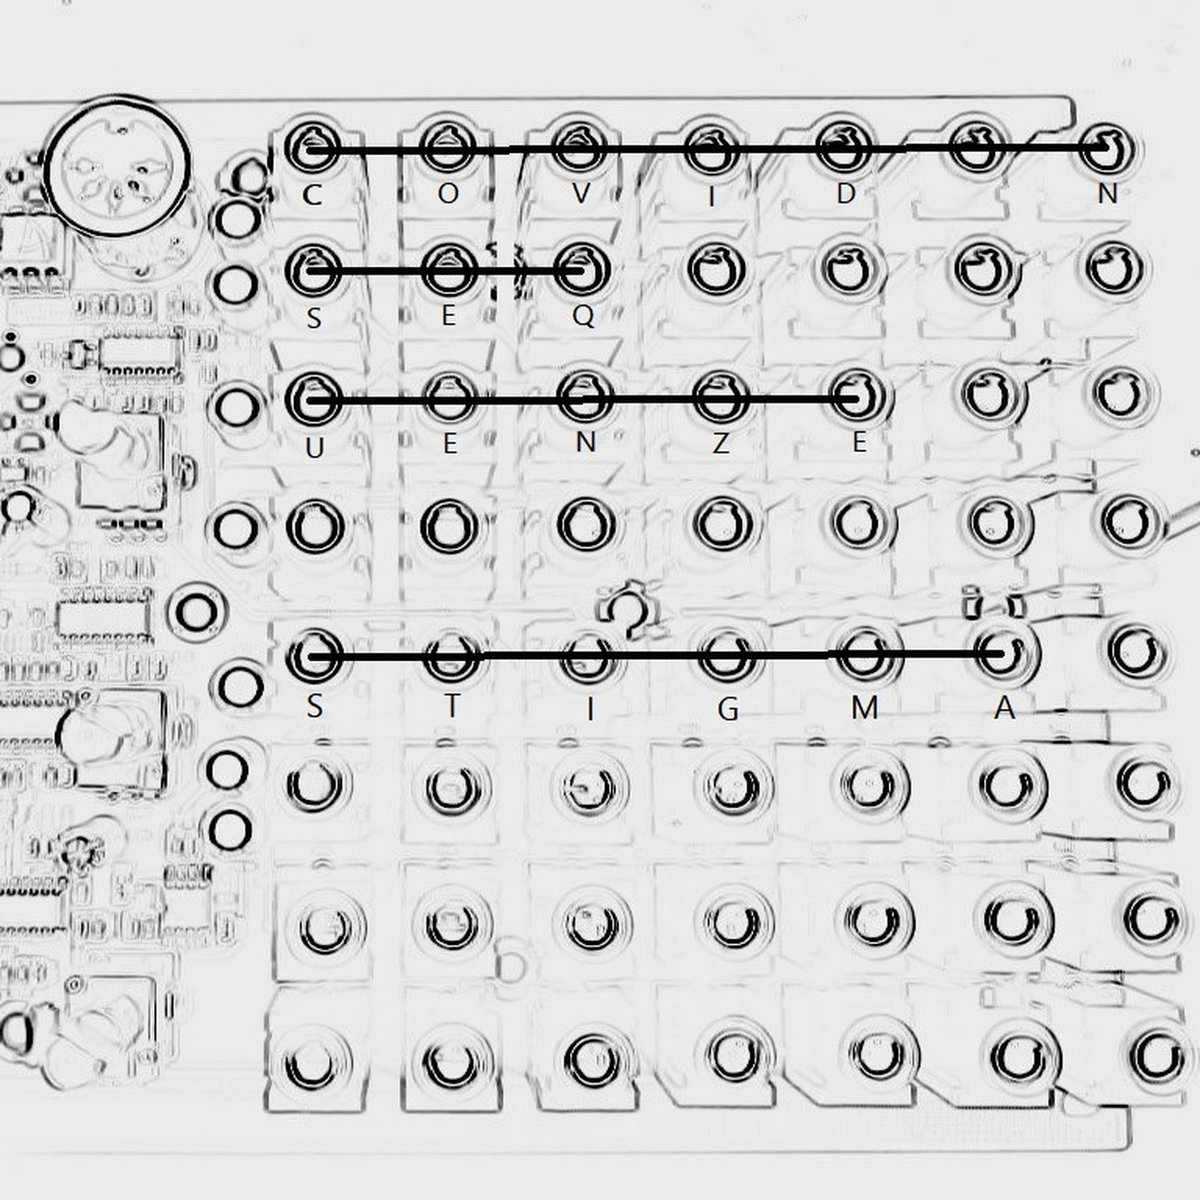
\includegraphics[width=8cm]{covidnsequenze.jpg}

\endminipage
\end{figure}

\clearpage

% ---------- New Chapter ----------

\section*{Skills}

Computer Music and Computer Science (DSP) with: 
\newline
Python, C, Arduino, LaTex, Lilypond, Pure Data,
Max Msp, Faust, CSound, ecc.
\newline
Computer Science and skills with: C, LaTex, Lilypond. Shell: Bash, CMD, ecc.
\newline
Musical Programming Microprocessors/Microcontrollers: Teensy, Arduino, Raspberry, ecc.
\newline
Mathematics of sounds, Acoustics and Psychoacoustics; analysis of environments and musical instruments
(Music information retrieval - MIR)
\newline
Basic experience in electrical engineering: Audio circuits, Analog synthesizers, Audio processing
\newline
Sound engineer, Mixing, Mastering. DAWs: Reaper, Ableton Live
\newline
Multimedia composition: Jitter(Max) and Processing.
\newline
History of Music and History of Electroacoustic Music; Musical analysis
\newline
Theory, rhythm and musical perception (solfeggio, ear training)
\newline
Compositional techniques: counterpoint, choral, contemporary
\newline
Musical Instrumental and Electroacoustic Composition
\newline
Basic experience with piano and keyboards; advanced with synthesizers

\begin{figure}[!htb]
\minipage{0.25\textwidth}
  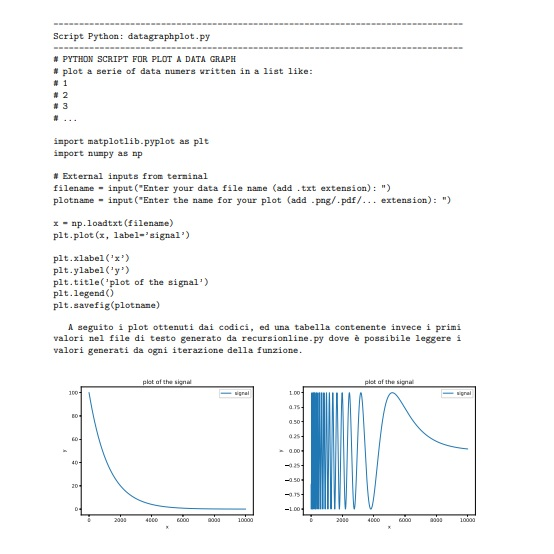
\includegraphics[width=8cm]{skills1.jpg}

\endminipage\hfill
\minipage{0.25\textwidth}
  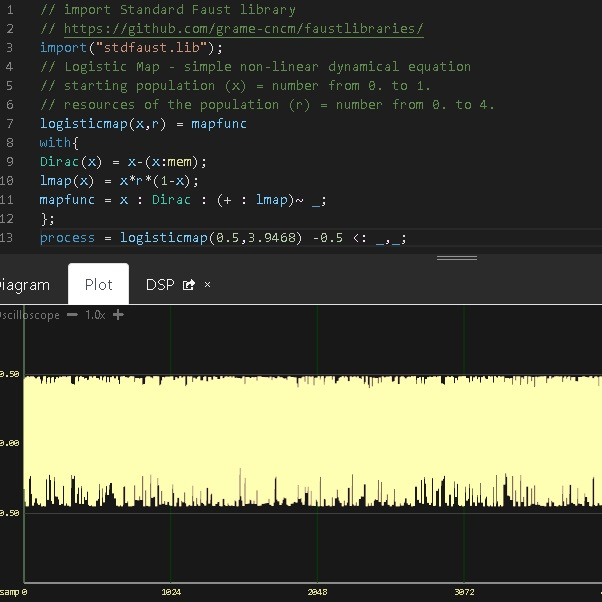
\includegraphics[width=8cm]{skills2.jpg}

\endminipage\hfill
\minipage{0.25\textwidth}%
  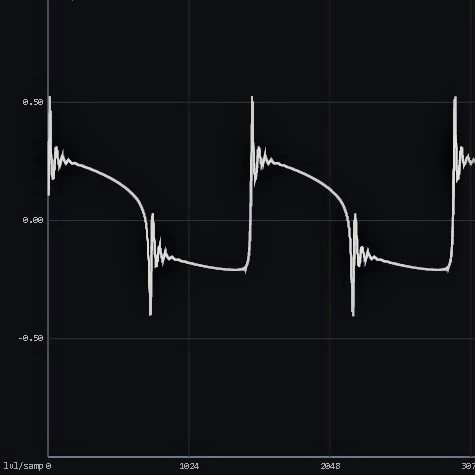
\includegraphics[width=8cm]{osc1.jpg}

\endminipage\hfill
\minipage{0.25\textwidth}%
  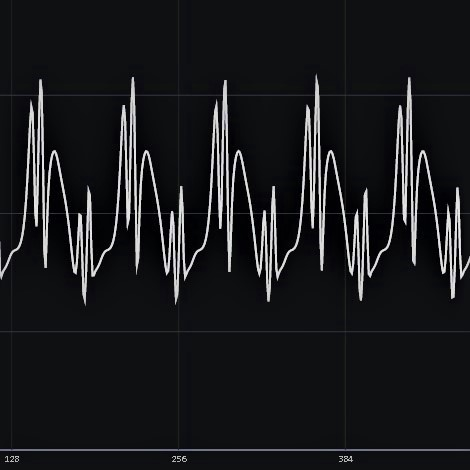
\includegraphics[width=8cm]{osc2.jpg}

\endminipage
\end{figure}

\clearpage

% ---------- New Chapter ----------

\section*{Researches and other links}

\begin{verbatim}
My personal links:
>Academia< https://conservatoriosantacecilia.academia.edu/LucaSpanedda
>Github< https://github.com/LucaSpanedda/
>Soundcloud< https://soundcloud.com/luca-spanedda-1995
>Youtube< https://www.youtube.com/channel/UCRCkVPYRcgo84G8W_uJZuaw
>Instagram< https://www.instagram.com/luca_spanedda/

Here you can find the links of the project STIGMA:
>Bandcamp< https://stigma-audio.bandcamp.com/
>Facebook< https://www.facebook.com/stigmaudio/
>Soundcloud< https://soundcloud.com/official-stigma-audio
>Youtube< https://www.youtube.com/channel/UCS3DHDatyEDVnrHCz5yvaig/featured
>Instagram< https://www.instagram.com/stigmaudio
\end{verbatim}

\clearpage

% HERE END THE TEXT -----------------------------------------------------------
\end{center}
}
\end{document}